% article example for classicthesis.sty
\documentclass[10pt,a4paper]{article} % KOMA-Script article scrartcl
\usepackage{import}
\usepackage{xifthen}
\usepackage{pdfpages}
\usepackage{transparent}
\newcommand{\incfig}[1]{%
    \def\svgwidth{\columnwidth}
    \import{./figures/}{#1.pdf_tex}
}
\usepackage{lipsum}     %lorem ipsum text
\usepackage{titlesec}   %Section settings
\usepackage{titling}    %Title settings
\usepackage[margin=10em]{geometry}  %Adjusting margins
\usepackage{setspace}
\usepackage{listings}
\usepackage{amsmath}    %Display equations options
\usepackage{amssymb}    %More symbols
\usepackage{xcolor}     %Color settings
\usepackage{pagecolor}
\usepackage{mdframed}
\usepackage[english]{babel}
\usepackage[utf8]{inputenc}
\usepackage{longtable}
\usepackage{multicol}
\usepackage{graphicx}
\graphicspath{ {./Images/} }
\setlength{\columnsep}{1cm}

% ====| color de la pagina y del fondo |==== %
\pagecolor{white}
\color{black}



\begin{document}
    %========================{TITLE}====================%
    \title{{  6th laboratory  }}
    \author{{Rodrigo Castillo}}
    \date{\today}

    \maketitle


    %=======================NOTES GOES HERE===================%
%    \section{ Read the introduction of the section 6 "Recognizing C Code
%        Constructs in Assembly" and explain what means a "Code Construct". What
%        aspects may impact the way as assembly code is generated?}
%        \color{red} this section is not supposed to be includded in laboratory \color{black}


%    \section{Read the section "Gobal vs Local Variables" and identify what are
%        the differences in the compilation of a code that employs global vs one
%        that employs local Variables.Ref: Section "Registers" Pag 104, Section "The Stack" Pag 110, Section "Stack
%        Layout" Pag 111. Section "C Main Method and Offsets" Pag 116.}
%        \color{red} this section is not supposed to be includded in laboratory \color{black}

    \section{operations :addition, substraction , increment, decrement and modulo}

        for addition:
        we can see that the addition operation is in line $ 666  $  , in
        operation $ add  $  , as i defined two variables before, assembly code
        is locating hex values into the variables i defined and then, he es
        adding the values into the new variable
        \begin{figure}[h!]
            \centering
            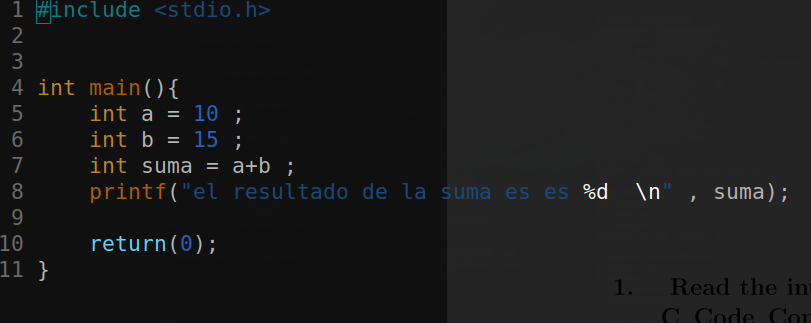
\includegraphics[width=1\linewidth]{codeforsum.png}
            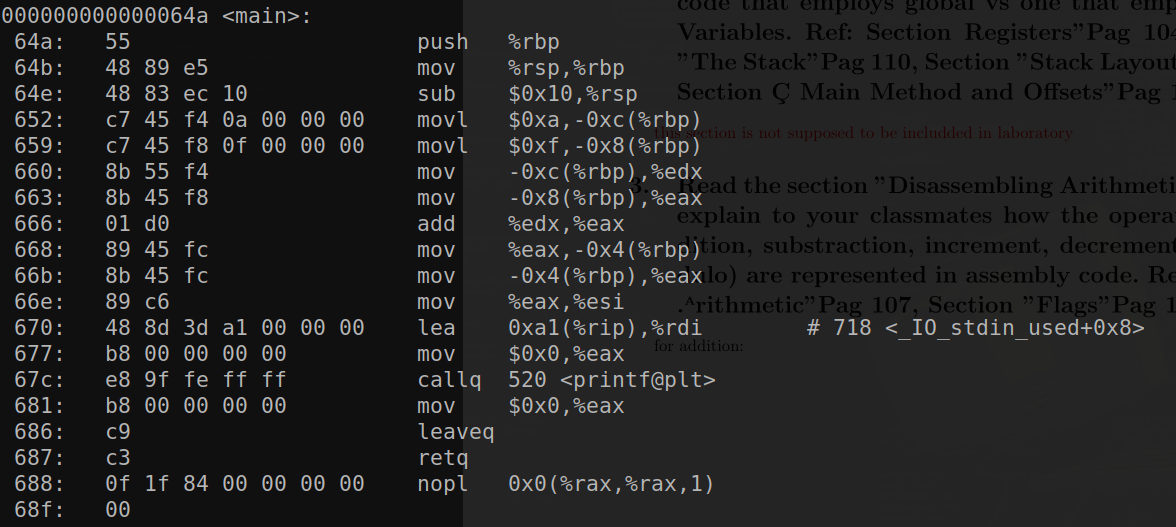
\includegraphics[width=1\linewidth]{sumadis.png}
            \caption{Code and disassembly for addition}
            \label{adfig}
        \end{figure}

        \newpage
        for substraction:
        this is the same as the addition operation, but, the code is replacing
        addition operation with substraction operation in line $ 663  $ .
        \begin{figure}[h!]
            \centering
            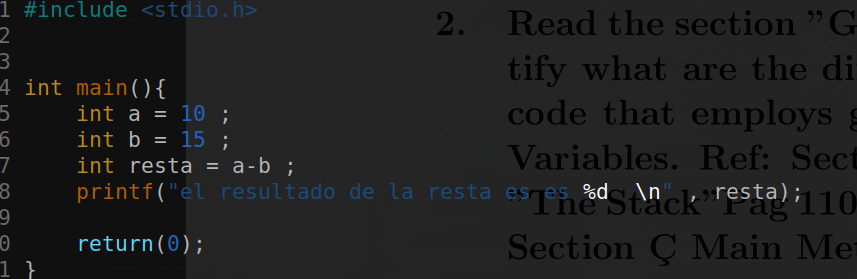
\includegraphics[width=1.0\linewidth]{codeforres.png}
            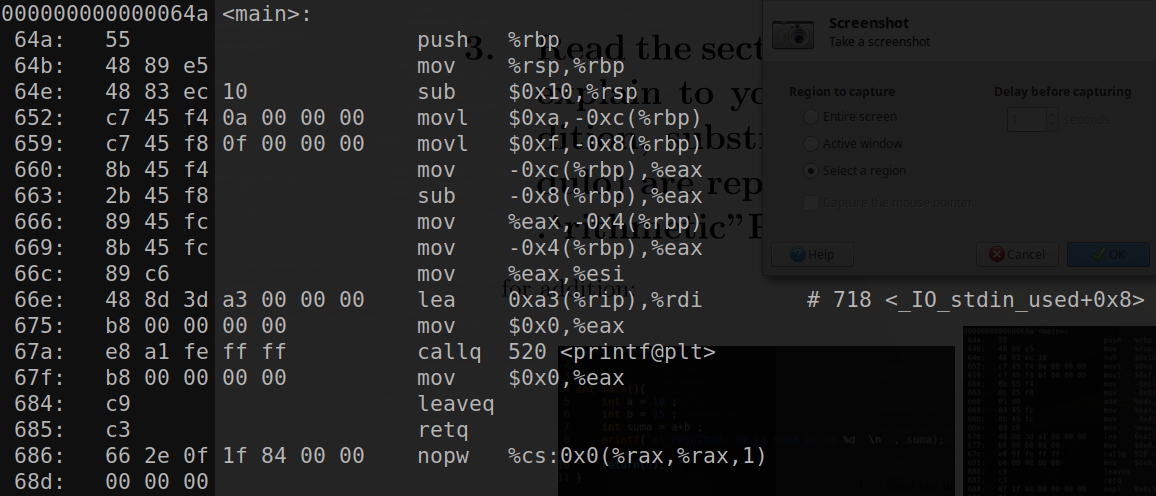
\includegraphics[width=1.0\linewidth]{resdis.png}
            \caption{Code and disassembly for substraction}
            \label{subfig}
        \end{figure}


        \newpage
        for increment:
        first, in line $ 652  $ we can see that is adding the value $ 0xa  $
        into a register, this value, is $ 10  $  , then its adding $ 0x1  $
        into the same register, this means that is adding 1 and now the value
        of this register is $ 11  $ .
        \begin{figure}[h!]
            \centering
            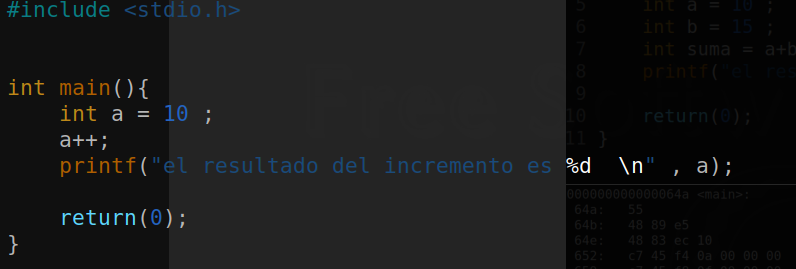
\includegraphics[width=1.0\linewidth]{codeinc.png}
            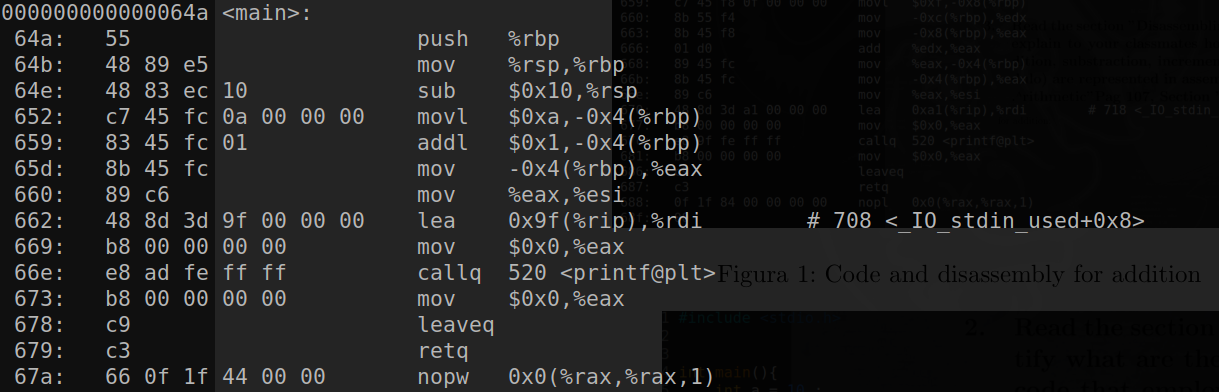
\includegraphics[width=1.0\linewidth]{incdis.png}
            \caption{Code and dissasembly for increment}
            \label{incfig}
        \end{figure}


        \newpage
        for decrement:
        is exactly the same as increment, but now, he es substracting instead
        of adding $ 0x1  $ value into the register.
        \begin{figure}[h!]
            \centering
            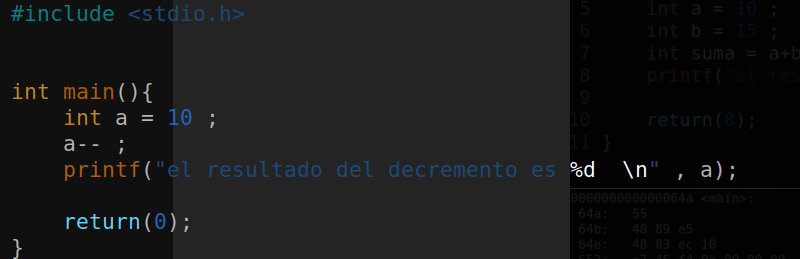
\includegraphics[width=1.0\linewidth]{deccode.png}
            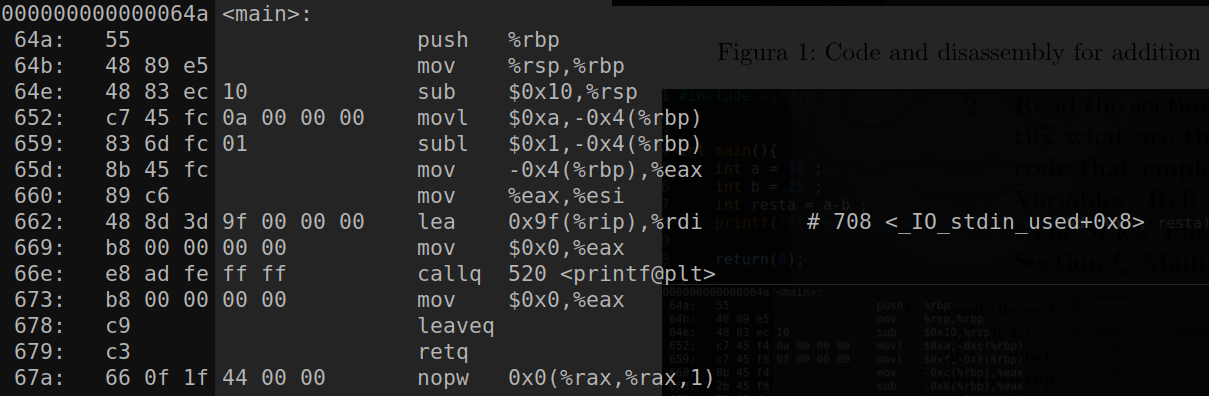
\includegraphics[width=1.0\linewidth]{decdis.png}
            \caption{Code and disassembly for decrement opperation}
            \label{figdec}
        \end{figure}

        \newpage
        for modulo:
        is actually the same as addition and substraction, but the opperation $
        idivl  $ stands for division, the result of this divion is going to
        store the residue in the designer register.
        \begin{figure}[h!]
            \centering
            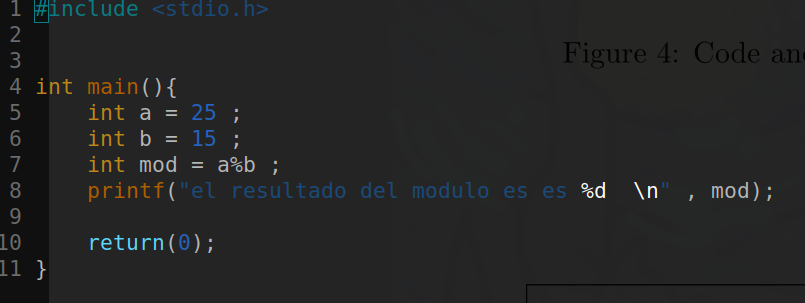
\includegraphics[width=1.0\linewidth]{modcode.png}
            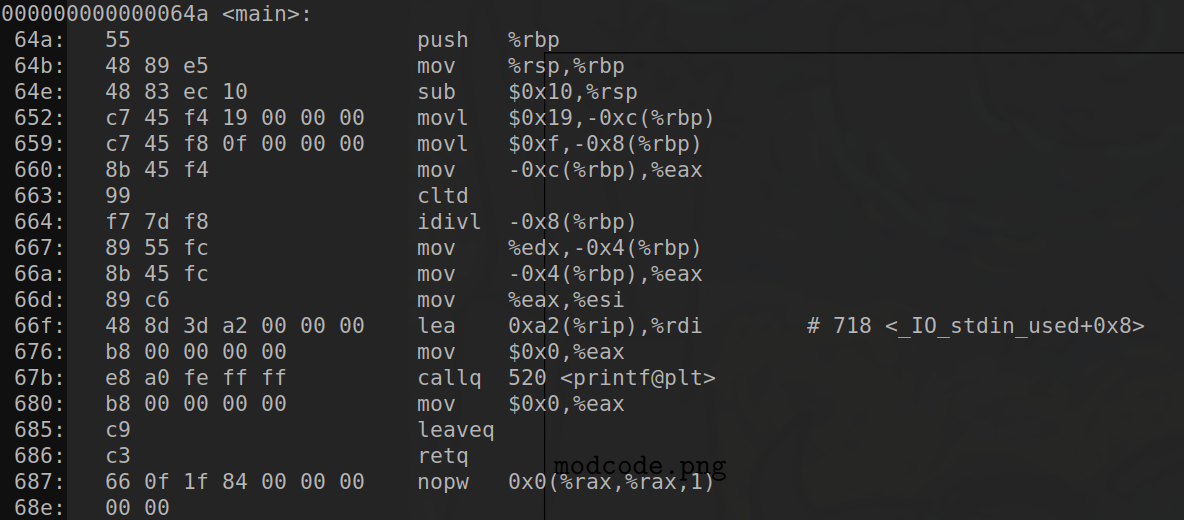
\includegraphics[width=1.0\linewidth]{moddis.png}
            \caption{Code for modulo}
            \label{figmode}
        \end{figure}







    \newpage
    \section{Q4: Read the section "Recognizing if Statements" and explain to
        your classmates how to recognize an if/else structure in assembly code.
        Ref: Section "Conditionals" Pag 113, Section "Branching" Pag 113}

        if statement in c:
        this disassemble, first, saves the variable 10 into the register, next,
        the compare instruction checks if the value in the register is equal to
        10, if is not equal , the instruction pointer is going to follow
        instruction $ 665  $ and substract, but if is equal, $ \$eip  $ is
        going to point at next instruction $ 65f  $ and add 1 to the register.
        \begin{figure}[h!]
            \centering
            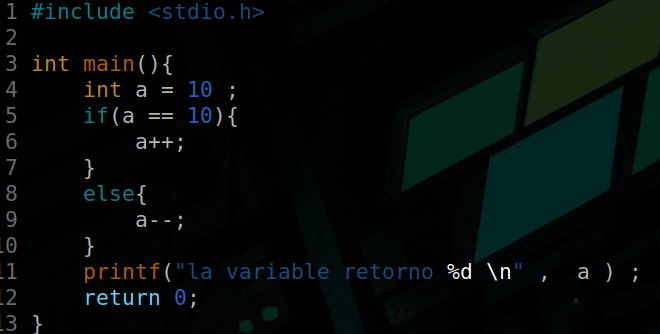
\includegraphics[width=0.9\linewidth]{ifcode.png}
            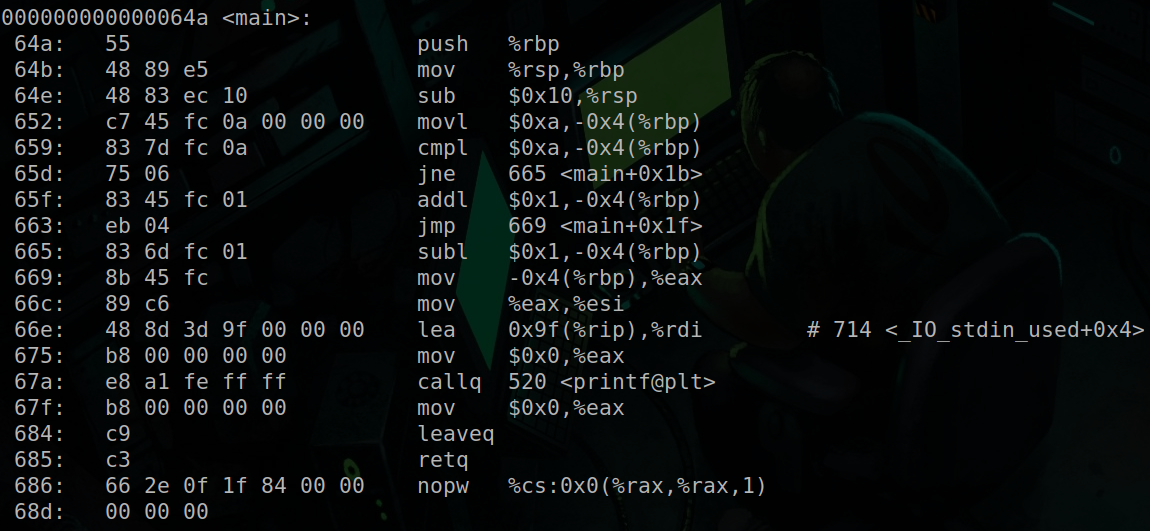
\includegraphics[width=0.9\linewidth]{ifdis.png}
            \caption{if statement and disassemble}
            \label{if}
        \end{figure}


    \newpage
    \section{Q5: Read the section "Recognizing Nested if Statements" and
        explain to your classmates how to recognize a "Nested IF" structure in
        assembly code.Ref: Section "Conditionals" and "Branching" Pag 113}

        nested:
        inside the memory spaces of the first $ jmp  $ instruction there are
        more $ jmp  $ instruction .
        \begin{figure}[h!]
            \centering
            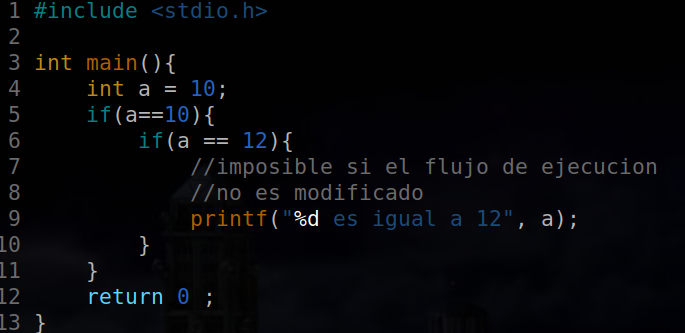
\includegraphics[width=0.9\linewidth]{nestedcode.png}
            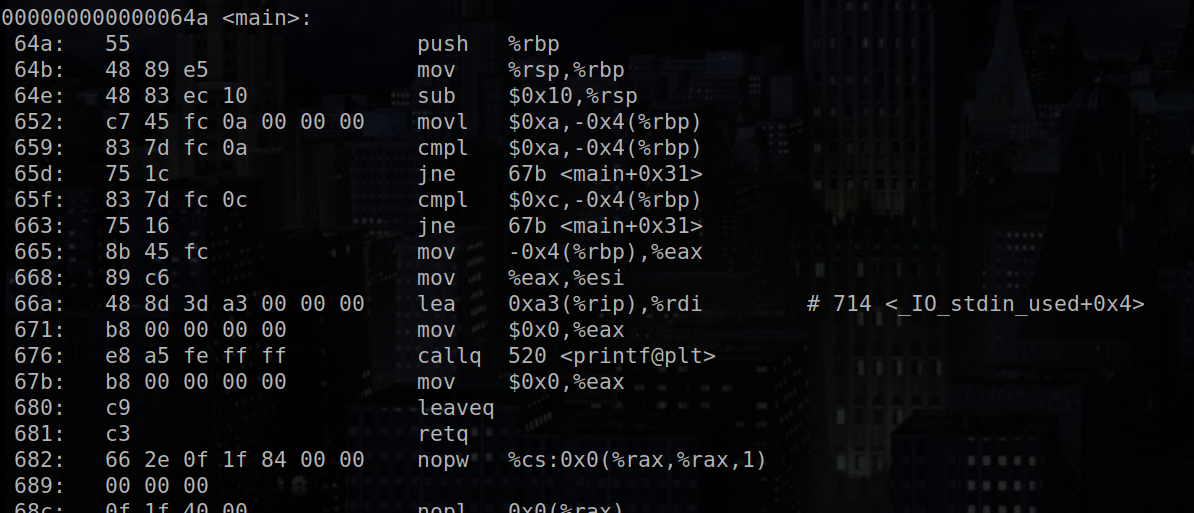
\includegraphics[width=0.9\linewidth]{nesteddis.png}
            \caption{Nested code and disassemble}
            \label{nested}
        \end{figure}

    \newpage
    \section{Q6: Read the section "Recognizing Loops" and explain to your
        classmates how to recognize a FOR structure in assembly code.
        Ref: Section "Conditionals" and "Branching" Pag 113}

        for:
        a for loop, in disassambly language, its the mix between an if and
        adittion instructions, here, we can see that the assembly code is
        executing print instruction. at first, he defines variable at 0 because
        in code, i = 0 , then it executes the instruction and then it compares
        the variable with 10, if the variable is equal to 10, follows normal
        flood of execution , but if variable is not equal to 10, it increases
        it by one and sets $ eip  $  to $ 65b  $ , that means that the program
        is going to execute this instruction 10 times until the variable $ i =
        10 $ .
        \begin{figure}[h!]
            \centering
            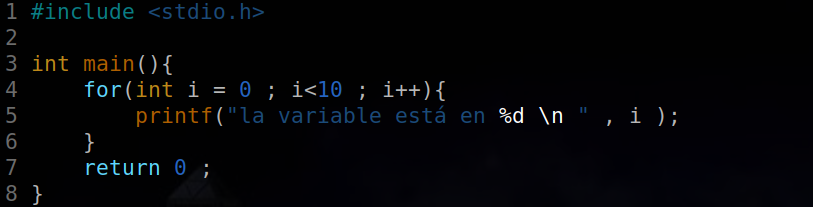
\includegraphics[width=0.9\linewidth]{forcode.png}
            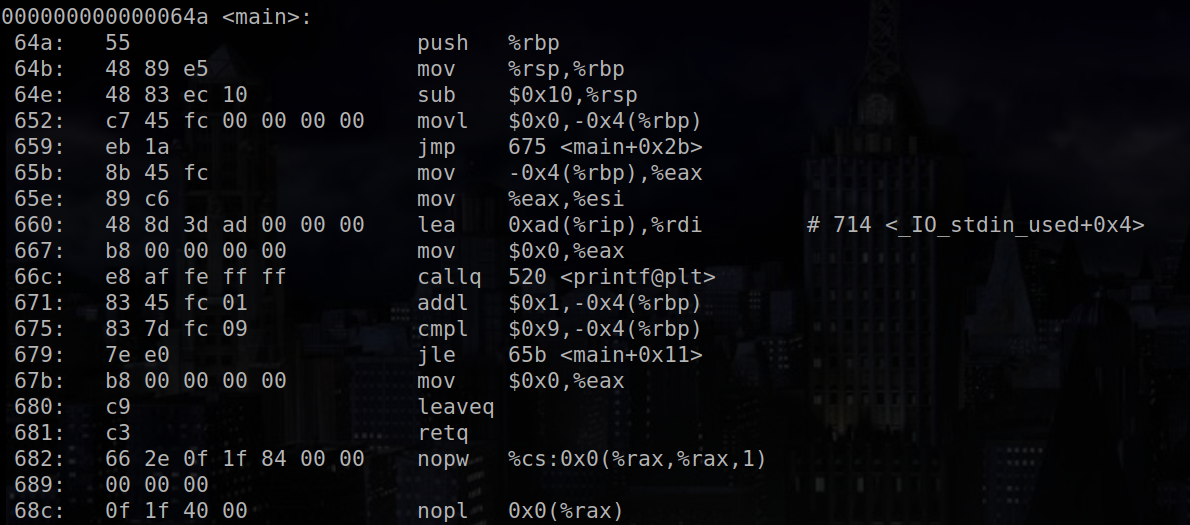
\includegraphics[width=0.9\linewidth]{fordis.png}
            \caption{For loop and disassemble}
            \label{for}
        \end{figure}

    \newpage
    \section{Q7: Read the section "Recognizing Loops" and explain to your
        classmates how to recognize a WHILE structure in assembly code.
        Ref: Section "Conditionals" and "Branching" Pag 113}

        while:
        while loop is similar to for loop, the difference is that its not going
        to increment anything if the code dont tell it to do , basically, in
        this example, its going to compare $ a  $ variable with $ 99= 0x63  $ ,
        if the comparisson returns true, the code is going to continue normal
        flood of execution, but if not, its going to set $ \$eip  $ to $ 0x663
        $ intruction, this means that its going to execute all the code again
        till the comparisson between $ a  $ and $ 0x63  $ returns true, by the
        way, this code is finit because in the instruction $ 678  $ i am adding
        1 to variable $ a  $ , but this is because i put it in the code, but
        this is not mandatory, this can make infinite loops .
        \begin{figure}[h!]
            \centering
            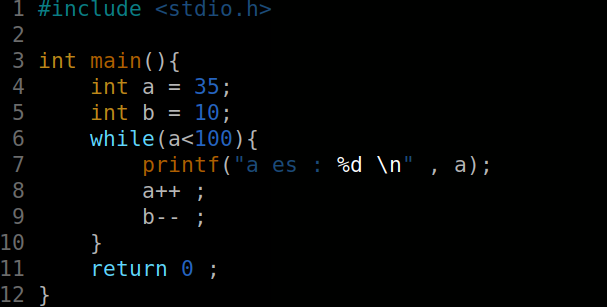
\includegraphics[width=0.8\linewidth]{whilecode.png}
            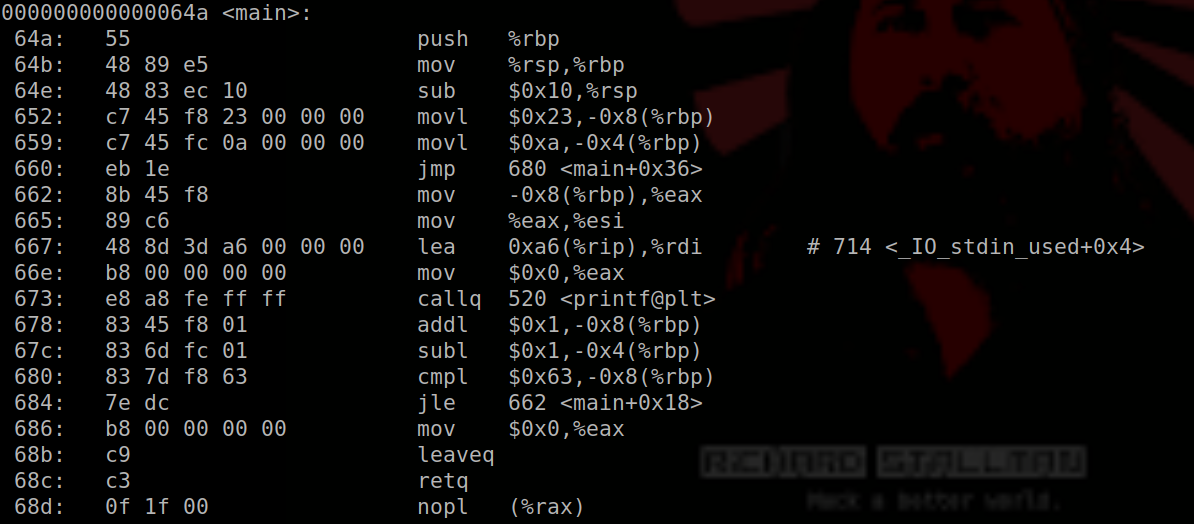
\includegraphics[width=0.8\linewidth]{whiledis.png}
            \caption{while code and disassemble}
            \label{while}
        \end{figure}

    \newpage
    \section{Q8: Read the section "Understanding Function Call Convenstions"
        and explain to your classmates how to recognize a "function call" in
        assembly code.
        Ref: Section "Function Calls" Pag 110. Section "Stack Layout" Pag 111. }

        function:
        calling a function into disassembly means that compiler is going to
        create another section for it with the name of the function in the code
        ,this will let the programmer call a function many times with only one
        definition. The processor is going to run the $ main  $ function by
        default, but,
        inside main function, the $ callq  $ intruction tells to execute the
        function inside the parameter, in this case we can see that the
        instruction is being called in $ 67e  $  , that means that in this
        space the pointer $ eip  $ is going to jump to $ 64a  $ where the
        function $ func  $ is allocated and its going to execute those
        intructions, the instructions in $ 64a $ section. when its done, the $
        retq  $ its going to return the $ eip  $ pointer to the original flood
        of execution in $ main  $ function.
        \begin{figure}[h!]
            \centering
            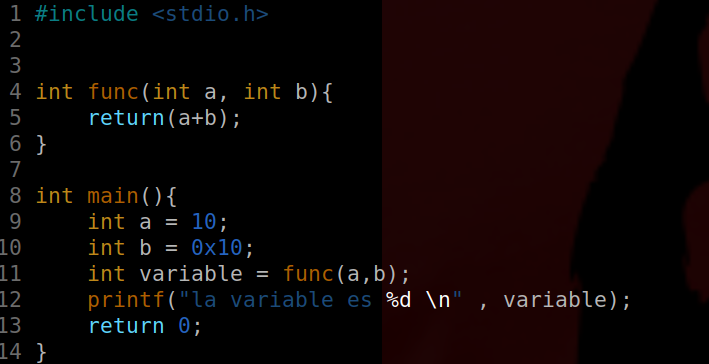
\includegraphics[width=0.8\linewidth]{funccode.png}
            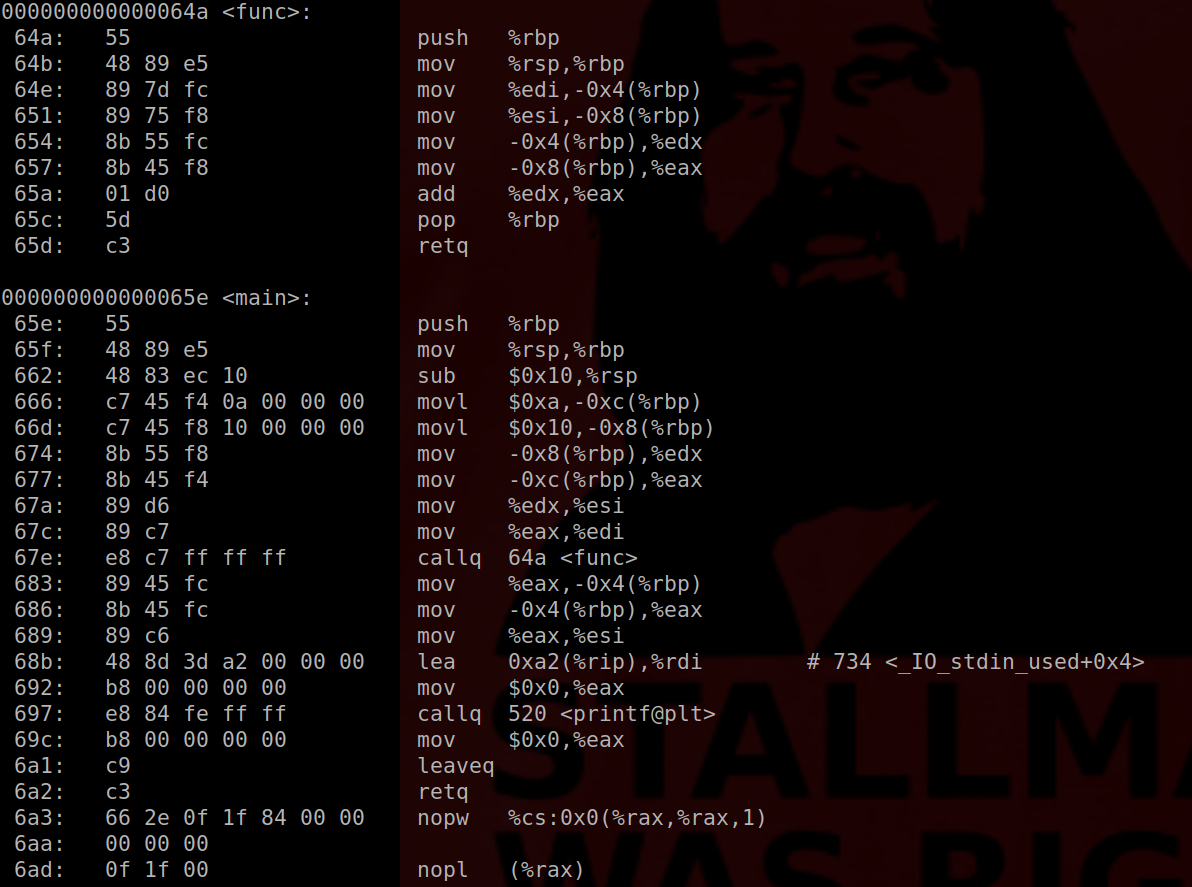
\includegraphics[width=0.8\linewidth]{funcdis.png}
            \caption{Function call and disassembly}
            \label{function}
        \end{figure}

    \newpage
    \section{Q9: Read the section "Analyzing switch Statements" and explain to
        your classmates how to recognize a switch structure in assembly code.}

        switch:
        switch is just a sequence of if-else statements , what assembly code is
        doing is concatenating  $ cmp  $ -  $ je  $(jump equal) intructions if
        the conditions are true al false. If the conditions are true, its going
        to run them, but if not, is going to set $ \$eip  $  to next $ cmp  $
        instruction, and its going to do this till the $ switch  $ statement is
        done .
        \begin{figure}[h!]
            \centering
            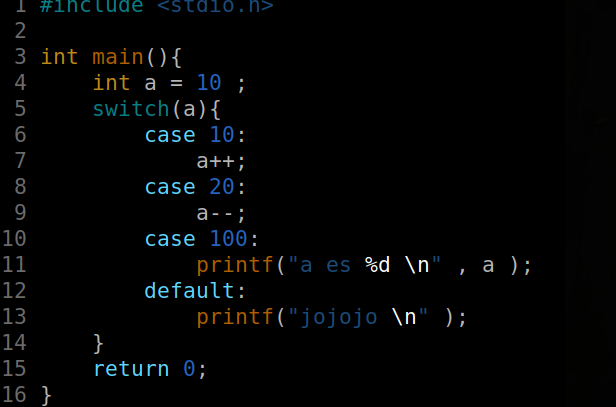
\includegraphics[width=0.8\linewidth]{switchcode.png}
            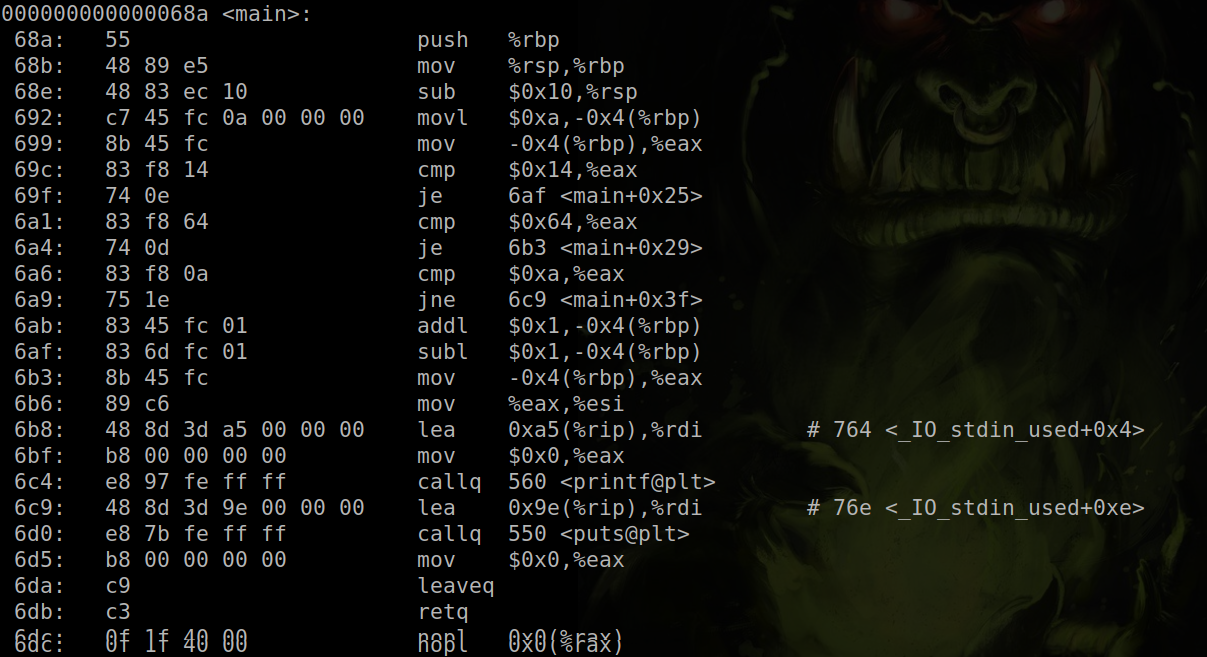
\includegraphics[width=0.8\linewidth]{switchdis.png}
            \caption{Switch disassemble}
            \label{switch}
        \end{figure}









    %=======================NOTES ENDS HERE===================%

    % bib stuff
    \nocite{*}
    \addtocontents{toc}{{}}
    \addcontentsline{toc}{section}{\refname}
    \bibliographystyle{plain}
    \bibliography{../Bibliography}
\end{document}
